% --------------------------------------------------------------
% This is all preamble stuff that you don't have to worry about.
% Head down to where it says "Start here"
% --------------------------------------------------------------
 
\documentclass[12pt]{article}
 
\usepackage[margin=1in]{geometry} 
\usepackage{amsmath,amsthm,amssymb, graphicx, verbatim}
 \usepackage{algorithm}
\usepackage{algorithmic}
\usepackage{hyperref}
\newcommand{\N}{\mathbb{N}}
\newcommand{\Z}{\mathbb{Z}}
 
\newenvironment{theorem}[2][Theorem]{\begin{trivlist}
\item[\hskip \labelsep {\bfseries #1}\hskip \labelsep {\bfseries #2.}]}{\end{trivlist}}
\newenvironment{lemma}[2][Lemma]{\begin{trivlist}
\item[\hskip \labelsep {\bfseries #1}\hskip \labelsep {\bfseries #2.}]}{\end{trivlist}}
\newenvironment{exercise}[2][Exercise]{\begin{trivlist}
\item[\hskip \labelsep {\bfseries #1}\hskip \labelsep {\bfseries #2.}]}{\end{trivlist}}
\newenvironment{problem}[2][Problem]{\begin{trivlist}
\item[\hskip \labelsep {\bfseries #1}\hskip \labelsep {\bfseries #2.}]}{\end{trivlist}}
\newenvironment{question}[2][Question]{\begin{trivlist}
\item[\hskip \labelsep {\bfseries #1}\hskip \labelsep {\bfseries #2.}]}{\end{trivlist}}
\newenvironment{corollary}[2][Corollary]{\begin{trivlist}
\item[\hskip \labelsep {\bfseries #1}\hskip \labelsep {\bfseries #2.}]}{\end{trivlist}}

\newenvironment{solution}{\begin{proof}[Solution]}{\end{proof}}
 
\begin{document}
 
% --------------------------------------------------------------
%                         Start here
% --------------------------------------------------------------
 
\begin{comment} 
Please include a section in your report detailing your GPU implementation, as well as its performance over varying numbers of particles. Here is the list of items you might show in your report:

A plot in log-log scale that shows the performance of your code versus the naive GPU code
A plot of the speedup of the GPU code versus the serial, openmp, mpi runs on the CPU of the node
A description of any synchronization needed
A description of any GPU-specific optimizations you tried
A discussion on the strengths and weaknesses of CUDA and the current GPU architecture
\end{comment}

\title{CS 267 Homework 3}
\author{Xingyou Song \footnote{xsong@berkeley.edu - Xingyou wrote the report, presented techniques and strategies for optimization, and coded some parts}, Yao Yuan \footnote{yao\_yuan@berkeley.edu - Yao coded a significant part of the code in C and tested using various compiler settings}, Jingbo Wu\footnote{wu622@berkeley.edu - Jingbo mainly contributed to the report and coding.}} %replace with your name
\date{March 23, 2018} 
\maketitle

\section{Algorithm}
For each rank, it calls upc++ $newarray$ function to allocate a shared global hashmap. After each process allocates their own global hashmaps, they broadcast the global address pointers to other ranks so that each rank is aware of others' global memory addresses. Besides, each rank creates a local LockerTable to make sure that no two ranks would try to write the same slot at the same time (race condition).

\subsection{Data Structures}
\begin{itemize}
\item Hash Map consists of n (number of ranks) global kmer arrays. Each rank is responsible for its own global arrays. 
\item Locker Table is a local char array for each rank. It is used to ensure that each corresponding slot in the global memory would only be written once (no duplicate write operations by different ranks). Whenever a rank try to insert its kmer into the global memory, it would first issue an rpc call the corresponding rank to require a valid slot. Only when the caller receives a success signal back from the other rank together with an assigned position, it would then do an rput operation. The locker table is implemented via C++ atomic or operation.
\end{itemize}

\subsection{insert\_kmer function}
In insert\_kmer, we do the following locally: 
\begin{itemize}
\item Compute a hash by calling kmer.hash(), and mod this by the size of the hash table to compute a position in the memory.
\item Compute which rank this position belongs to, and the relative address of the rank's global memory (respectively, variables whichProc and whichSlot). Issue a rpc command to the corresponding rank to check if the corresponding slot is open.
\item Use C++ atomic function to check whether the corresponding slot is open or not. If not, use linear probing to probe the next slot until an empty slot is found. If all the rank's slots are full, a "Not Found" message is returned to the rpc caller and the caller would issue another rpc insert kmer command to the next rank. This process is repeated until an open slot is found. One thing that is worth mentioning is that there are at most up to the number of ranks RPC calls for one insertion operation.
\item If we succeed in finding an open slot, insert this globally. 
\end{itemize}
\subsection{find\_kmer function}
We will also do the following for find\_kmer: 
\begin{itemize}
\item Compute the hash and position, like we did with insert\_kmer. 
\item Retrieve a kmer using rget() function. If it is not equal to the key, increment the probe variable by 1 (which moves the position by 1), and continue checking until success or we go over the hash\_map limit. 
\end{itemize}
Note that when we initialize, we collect all of the meta data (i.e. size of each processor's collection, their ranks, their global hash map pointers etc.) by a master call, with this passed as a global pointer to each processor. 


\subsection{Explanation}
There are multiple ways to do this, but because of the hash collision nature, it was only sensible to split the memory to be allocated for nodes, and take the communication penalty for when a hash belongs to another node's memory, which is perfect for the UPC++ case. Besides, we do a greedy probing algorithm within one rank's locker table to minimize the number of rpc functions. 


\section{Results}

\subsection{Single Node, Varying Processes}
\ref{graph1}
From our results, we see that the strong scaling for all datasets are very similar. The strong scaling has a steep drop for few processes on a single node, most likely because the overhead of communication is too significant to be neglected. However, we see the slope is rather flat when we have more than 4 ranks. One possible explanation is that the extra communication overhead is offset by the distributed workload. (the number of rpc calls per insertion is always around 1-2. So the more evenly distributed the workload is, the more efficient the code is). 
On average, we have a scaling efficiency of 0.48.
\subsection{Multi Node}
\ref{graph2} For the multi-node case, the scaling remains similar for all datasets. Again, we see a very sharp drop in scaling due to both collision overheads and node-communication (based on the hash assigned to different nodes). 

Note that there is a strange peak at nodes = 2 for all test cases; this is the beginning of multi-node parallelization, and it suggests that communication complexity between nodes (through the ethernet) dominates when we start parallelization. 

Also, note that for this graph, we don't see significant speed-up for extra nodes, which is possibly explained by two reasons.

Firstly, as the whole hash map is further divided into small chunks when the number of ranks increases and the linear probing method tends to suffer from clustering. It is highly possible that some rank's hash maps might be full really early in the insertion procedure, thus suffering from long probing time (kind of similar to a naive for loop).

Secondly, the access of other nodes' global memory is not cheap at all. Compared to rget / rput on a single node across different ranks, doing rget / rput remotely from another single node suffers from large communication overhead. To mitigate the issue, one possible solution is to create some minibatch or the requests so that we can better make use of the TCP packets padding, thus reducing communication overhead.
On average, we have a scaling efficiency of 0.24.


\begin{figure}[h] 
  \caption{Single Node, Varying Processes}
  \centering 
  \label{graph1}
  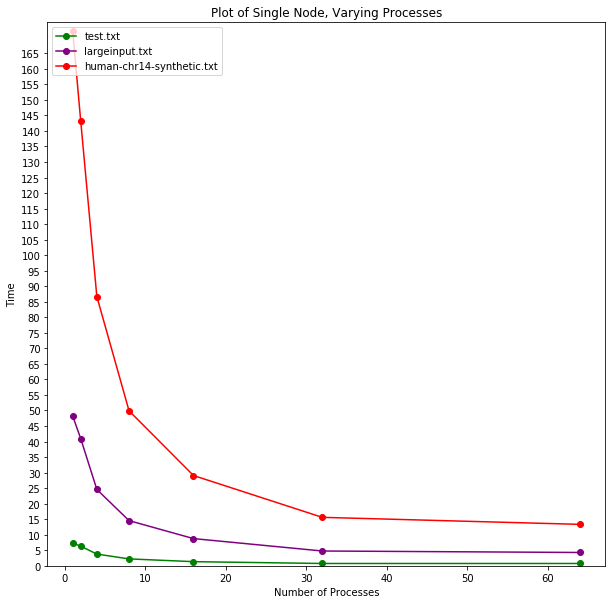
\includegraphics[width = 0.65\textwidth]{single_node.png}
  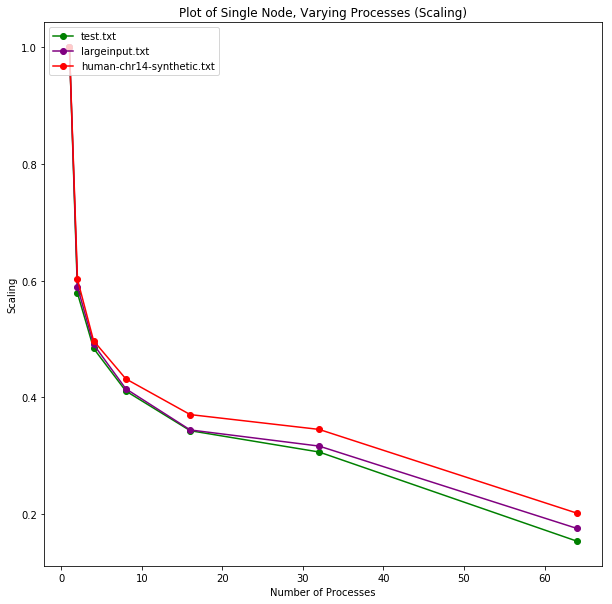
\includegraphics[width = 0.65\textwidth]{single_node_scaling.png}
\end{figure}


\begin{figure}[h]
  \caption{Multi-Node, 32 Ranks Per Node}
  \centering 
  \label{graph2}
  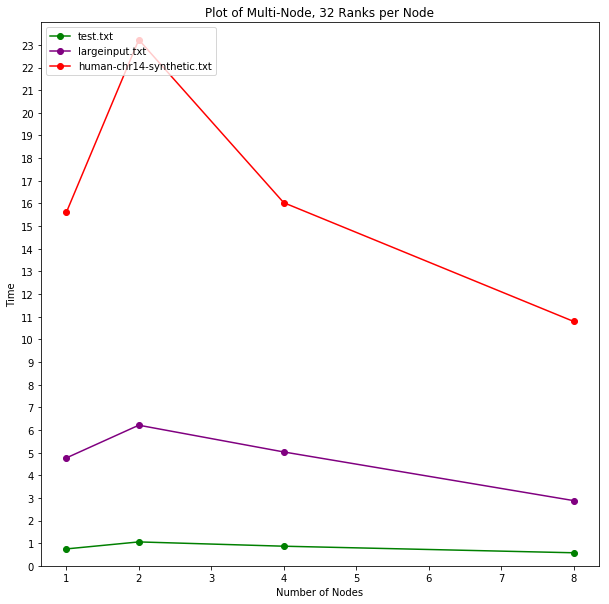
\includegraphics[width = 0.65\textwidth]{multi_node.png}
  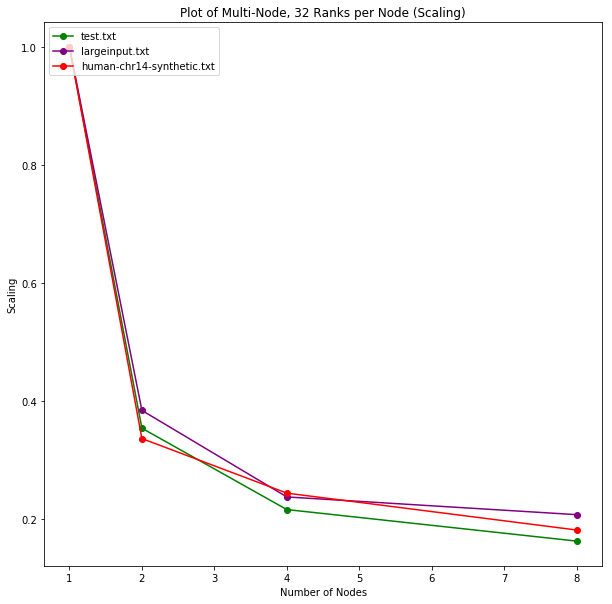
\includegraphics[width = 0.65\textwidth]{multi_node_scaling.png}
\end{figure}

\section{Other frameworks}
In other frameworks, we run into the same architecture as before - we must assign each memory "worker" (either a thread or process) to its own unique set of memory locations; this is the cleanest way to do so, or else there will be very large memory conflict overheads requiring locks (i.e. who writes first, and who reads first on the same location?)
\subsection{MPI} 
In the MPI setting for synchronized and parallelized hashing, the clearest way to do so is to allow each processor hold a section of memory for the hash table, just like we did with UPC++. However, there is a problem when it comes to communication: i.e. when one processor detects that the hash position value does not correspond to its own memory location, it must pass this signal to the correct processor (which is not known ahead of time), which forces all of the processors to wait for a message (about whether they do nothing, or need to perform a memory insert). A similar problem exists for the find\_kmer function.

Perhaps a better method exists, where we allocate a few processors (called the masters) to process the parallelized hashing requests, and send the memory requests to the "worker" processors for memory operations. The problem with this occurs when two master processors send in 2 work requests to a worker at the same time, making synchronization difficult. 

\subsection{OpenMP} For OpenMP, each thread possesses its own memory locations in a global memory. A similar problem exists as seen above - even if we had "master" threads to control the flow of memory requests, there would be multiple synchronization issues, requiring many barriers, which decreases performance. 

\section{Bonus Questions}
\subsection{Short Answer - Contig F Extensions}
Then it will be impossible to know where to start and where to end. In other words, we need to have a separate list telling us which kmer is the starting point and which kmer is the end point. 
If there is a random base whose kmer is not within our dataset, we have two options. We can either pretend there is one (as we know what that kmer should be) or we just abort the generation of that kmer. In other words, we discard the half-complete kmer and move to the next one. It will not affect my code a lot as the hash map find function will return false if the kmer is not within the dataset and we can simple continue the iteration over the start\_kmers  while aborting the current contig.

\subsection{Short Answer - Load Balancing}
The idea behind it is to distribute the workload evenly. One simple approach is to let assign a single process as the coordinator and collect all the start\_nodes from other peers (including its own). Then, it can evenly split the start\_nodes and distribute them to other processes. It is easy to implement but might not be time efficient as a process has to receive and distribute all the start\_nodes. 





\begin{comment}
\subsection{Results}
\begin{figure}[h]
  \caption{GPU Final Code vs GPU naive (Avg Speed up 35.29, GPU final log-log slope avg is 0.20}
  \centering 
  \includegraphics[width = 0.65\textwidth]{GPU_final_vs_GPU_naive.png}
  \includegraphics[width = 0.65\textwidth]{GPU_final_vs_Serial_final.png}
\end{figure}



\section{Results}
We present our results (every processor only has one thread): 

\begin{table}[h]

\begin{tabular}{||c c c||} 
 \hline
 Particles & Avg Strong Scaling & Avg Weak Scaling  \\ [0.5ex] 
 \hline\hline 
 %%%%%%%%%%
 500 & 0.27 & 0.49 \\
 \hline 
 1000 & 0.31 & 0.40 \\
 \hline 
 1500 & 0.31 & 0.41  \\
 \hline
%%% DO NOT TOUCH PLS 
\end{tabular}

\end{table}
\begin{table}[h]

 \begin{tabular}{||c c c||} 
 \hline
 Particles & Processor & Time (s)  \\ [0.5ex] 
 \hline\hline
 500 & (Serial) & 0.081663 \\
 \hline 
 500 & 1 & 0.095706  \\
 \hline
  500 & 2 & 0.07736  \\
 \hline
  500 & 4 & 0.104709  \\
 \hline
  500 & 6 & 0.078448  \\
 \hline
  500 & 12 & 0.107769  \\
 \hline
  500 & 16 & 0.080899  \\
 \hline
  500 & 24 & 0.104492   \\
 \hline
  500 & 32 & 0.096736  \\
 \hline
  1000 & 2 & 0.129597  \\
 \hline
  2000 & 4 & 0.237802  \\
 \hline
  3000 & 6 & 0.232805  \\
 \hline
  6000 & 12 & 0.362595  \\
 \hline
  8000 & 16 & 0.504432  \\
 \hline
  12000 & 24 & 0.520144  \\
 \hline
 %%%%%%%%%%%%%
%%% DO NOT TOUCH PLS 
\end{tabular}
\begin{tabular}{||c c c||} 
 \hline
 Particles & Processor & Time (s)  \\ [0.5ex] 
 \hline\hline 
 %%%%%%%%%%%%%
 1000 & (Serial) & 0.169638 \\
 \hline 
 1000 & 1 & 0.183064 \\
 \hline 
 1000 & 2 & 0.129295 \\
 \hline  
 1000 & 4 & 0.128382 \\
 \hline 
 1000 & 6 & 0.121484 \\ 
 \hline  
 1000 & 12  & 0.121381 \\
 \hline 
 1000 & 16 & 0.120848 \\ 
 \hline  
 1000 & 24 & 0.133204 \\
 \hline 
 1000 & 32 &  0.13395 \\ 
 \hline 
 2000 & 2 & 0.249004 \\
 \hline 
 4000 & 4 & 0.379472 \\
 \hline 
 6000 & 6 & 0.690608 \\ 
 \hline 
 12000 & 12 & 0.635974 \\
 \hline 
 16000 & 16 & 0.70321 \\
 \hline 
 24000 & 24 & 0.810816 \\
 \hline 
 32000 & 32 & 0.842401 \\
 \hline 
 %%%%%%%%%%

%%% DO NOT TOUCH PLS 
\end{tabular}
\end{table}
\begin{table}
\begin{tabular}{||c c c||} 
 \hline
 Particles & Processor & Time (s)  \\ [0.5ex] 
 \hline\hline 
 %%%%%%%%%%
 1500 & (Serial) & 0.25489 \\
 \hline 
 1500 & 1 & 0.284891 \\
 \hline 
 1500 & 2 & 0.196361  \\
 \hline  
 1500 & 4 & 0.183619 \\
 \hline 
 1500 & 6 & 0.164744  \\ 
 \hline  
 1500 & 12  & 0.139465 \\
 \hline 
 1500 & 16 & 0.158564  \\ 
 \hline  
 1500 & 24 &  0.14834 \\
 \hline 
 1500 & 32 &  0.169517 \\ 
 \hline 
 3000 & 2 & 0.369944  \\
 \hline 
 6000 & 4 &  0.739809  \\
 \hline 
 9000 & 6 & 0.736118 \\ 
 \hline 
 18000 & 12 & 0.938799 \\
 \hline 
 24000 & 16 & 0.937171 \\
 \hline 
 36000 & 24 & 1.09924 \\
 \hline 
 48000 & 32 & 1.23157  \\
 \hline 
%%% DO NOT TOUCH PLS 
\end{tabular}

\end{table} 

\clearpage 

\subsection{Performance}
Note that when we fix the particle size and vary the number of processors, the curve becomes slightly smoother. At 500 points, we see that there is no clear sign of monotonicity, while at 1500 points, we see that our performance increases as the number of processors increases, but performance decreases at 20-32 processors. We seem to only see the $O(n/p)$ performance when the number of processors is between 5-15. This shows that communication overhead becomes a significant factor in designing the simulation. 
\\ \\ 
However, when we vary the number of particles with the number of processors, our performance becomes asymptotic as the time seems to be reaching an asymptotic limit - This suggests that for both large $n$ and $p$, we are also reaching a $O(n/p)$ asymptotic performance. Since at 1500 particles/processor, the log of time slightly increases, this means that there is a slight dominance of the number of particles - e.g. our asymptotic time could possibly be more similar to $O(n^{1 + \epsilon}/p)$ where $\epsilon > 0$, which makes sense as more particles imply more boundary changes, which implies more memory communication between processors, which has a much worse performance scaling than pure computation. 
\clearpage 

\begin{figure}[h]
  \caption{Fixed Particle Sizes, Varying Processor}
  \centering 
  \includegraphics[width = 0.65\textwidth]{500_fixed_particles_varying_processor.png}
  \includegraphics[width = 0.65\textwidth]{1000_fixed_particles_varying_processor.png}
  \includegraphics[width = 0.65\textwidth]{1500_fixed_particles_varying_processor.png}
\end{figure}


\begin{figure}[h]
  \caption{Varying Particle Size with Processor}
  \centering
    \includegraphics[width = 0.65\textwidth]{500_varying_particles_varying_processor.png}
  \includegraphics[width = 0.65\textwidth]{1000_varying_particles_varying_processor.png}
  \includegraphics[width = 0.65\textwidth]{1500_varying_particles_varying_processor.png}
 
\end{figure}

\clearpage
\subsection{Doing Better?}
We attempted other variants of MPI, including as mentioned, different shapes for the "sector" used by each processor. We may possibly see different results if, for example, processors which are assigned to the outer blocks of the grid are larger, specifically because particles bounce back from the wall on the outer edge, requiring less communication. 
\\ \\
Another optimization considered is the communication architecture used as well - we found that including a master processor which controls the synchronization of the worker processors resulted in a slow down. It is possible that we could, instead of enforcing every worker processor to signal all of the other worker processors its completion, we divide the grid into e.g. 2 groups, with 2 masters - this way all processors belonging to a group may only signal his completion to the corresponding master, and allow synchronization between the two masters. This setting would be more appropriate for 2 dense regions that are not connected well. 
% --------------------------------------------------------------
%     You don't have to mess with anything below this line.
% --------------------------------------------------------------
 \end{comment}
\end{document}
